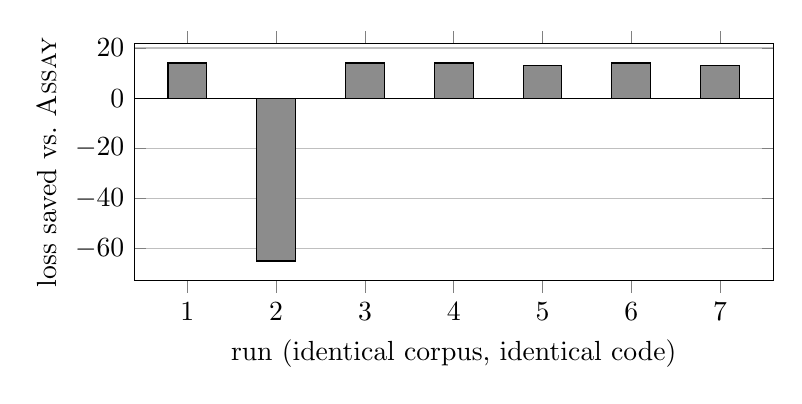
\begin{tikzpicture}
\begin{axis}[ybar, width=0.8\linewidth, height=4.6cm, xlabel={run (identical corpus, identical code)},
  ylabel={loss saved vs.\ \textsc{Assay}}, xtick={1,...,7}, ymajorgrids, bar width=14pt, enlarge x limits=0.1]
\addplot[fill=black!45] coordinates {(1,14.0) (2,-65.0) (3,14.0) (4,14.0) (5,13.0) (6,14.0) (7,13.0)};
\draw[black] (axis cs:0.4,0) -- (axis cs:7.6,0);
\end{axis}
\end{tikzpicture}
